\documentclass[aspectratio=169]{beamer}

\usetheme[numbering=fraction,progressbar=frametitle]{metropolis}
\usecolortheme{spruce}
\usepackage[utf8]{inputenc}
\usepackage[T1]{fontenc}
\usepackage{microtype}
\usepackage{graphicx}
\usepackage{booktabs}
\usepackage{hyperref}
\usepackage{wrapfig}
\usepackage{tikz}
\usetikzlibrary{shapes.geometric,calc}
\graphicspath{{figures/}}

\hypersetup{
  colorlinks=true,
  linkcolor=royal,
  urlcolor=accent,
  citecolor=royal
}

\definecolor{royal}{HTML}{0F4C5C}   % deep teal-blue
\definecolor{accent}{HTML}{F26430}  % modern orange
\definecolor{mint}{HTML}{5FB7B7}    % soft teal accent
\definecolor{violet}{HTML}{6C63FF}
\definecolor{softbg}{HTML}{F6F2EA}  % warm neutral background
\definecolor{danger}{HTML}{DD614A}

\metroset{
  background=light,
  block=fill,
  titleformat=smallcaps
}

\setbeamercolor{palette primary}{bg=royal,fg=white}
\setbeamercolor{normal text}{fg=royal,bg=softbg}
\setbeamercolor{frametitle}{bg=royal,fg=white}
\setbeamercolor{progress bar}{fg=accent,bg=accent!25!white}
\setbeamercolor{block title}{bg=royal,fg=white}
\setbeamercolor{block body}{bg=white,fg=royal}
\setbeamercolor{alerted text}{fg=danger}

\setbeamertemplate{background}{%
  \begin{tikzpicture}[remember picture,overlay]
    \path[fill=softbg] (current page.south west) rectangle (current page.north east);
  \end{tikzpicture}%
}

\newcommand{\metric}[3][]{%
  \begin{minipage}[t]{#2}\raggedright
    {\Large\bfseries\textcolor{accent}{#3}}\\[-0.2em]
    {\scriptsize #1}
  \end{minipage}}
\newcommand{\callout}[2]{\textbf{\textcolor{accent}{#1}}\,\,\textcolor{royal}{#2}}

\newcommand{\leftlogo}{./logos/observatory_400x332.jpg}
\newcommand{\midlogo}{./logos/silso-logo.png}
\newcommand{\rightlogo}{./logos/BELSPO_1867x1563.jpg}

\setbeamertemplate{section page}{%
  \begin{centering}
    \vfill
    {\color{royal}\Large\bfseries \insertsection}\par
    \rule{0.3\linewidth}{1pt}\par
    \vspace{0.4em}
    {\color{accent}\small Sunspot Number Next-Gen}
    \vfill
  \end{centering}}

\AtBeginSection{
  \sectionpage
}

\title{\textcolor{royal}{Refining the Sunspot Number Series to SN~V3}}
\subtitle{\textcolor{royal}{Reconstructing a Provenance-Rich Solar Activity Record}}
\author[FarSuN Team]{Kalugodu Chandrashekhar$^{1}$ \and Laure Lef\`evre$^{1}$ \and Benjamin Mampaey$^{1}$ \\
Senthamizh Pavai Valliappan$^{1}$ \and Hisashi Hayakawa$^{2}$ \and Christian Ritter$^{3}$}
\institute[ROB / SILSO]{\scriptsize $^{1}$ Royal Observatory of Belgium (ROB) / SILSO\quad $^{2}$ Nagoya University\quad $^{3}$ Universit\'e Catholique de Louvain, ISBA, LIDAM}
\date{ESWW 2025}
\titlegraphic{\vspace{6.8cm}\includegraphics[height=1.0cm]{\leftlogo}\hfill\includegraphics[height=1.0cm]{\midlogo}\hfill\includegraphics[height=1.1cm]{\rightlogo}}

\begin{document}

% --- Title ---
\begin{frame}
  \titlepage
\end{frame}

\begin{frame}[t]{Session Overview}
\begin{columns}[T,onlytextwidth]
\column{0.52\linewidth}
\textbf{We will cover}
\begin{itemize}
  \item Why the Sunspot Number needs a ground-up reconstruction.
  \item FARSuN's four-axis workflow and quality gates.
  \item Highlights from key historical datasets driving SN~V3.
  \item Expected benefits, community roadmap, and ways to engage.
\end{itemize}

\column{0.44\linewidth}
\textbf{Reference material}
\begin{itemize}
  \item FARSuN interactive report (webpage.html).
  \item ESWW25 posters: FARSuN Reconstruction \& SN Next-Gen.
  \item Dataset dossiers (QMD files) for Zürich, Mittheilungen, Adams, Gruithuisen, Stark.
\end{itemize}
\end{columns}
\end{frame}

\section[Mission]{Mission Brief}

\begin{frame}[t]{Why FARSuN?}
\small
The Sunspot Number (SN, formerly the International Sunspot Number) underpins space climate diagnostics, yet two major recalibrations still leave observer-dependent jumps (e.g. the 1947 "Waldmeier break").\linebreak[1]

\medskip
FARSuN (Findability and Accessibility of historical Raw Sunspot Numbers) is rebuilding the index from primary sources (1607--1980) with traceable metadata, uncertainties, and open delivery.

\vspace{0.6em}
\begin{columns}[T,onlytextwidth]
\column{0.5\linewidth}
\callout{Mission}{Recover and standardise dispersed sunspot archives (drawings, tables, weather notes).}

\column{0.5\linewidth}
\callout{Outcome}{Deliver SN~V3 with hemispheric indices, provenance, and FAIR-compliant access.}
\end{columns}
\end{frame}

\begin{frame}[t]{Project Pulse (Early 2025)}
\vspace{-0.2em}
\begin{columns}[T,onlytextwidth]
\column{0.33\linewidth}
\metric[Temporal coverage of curated sources]{\linewidth}{1607--1980}
\par\vspace{0.8em}
\metric[Zürich observation tables digitised (Transkribus + manual QC)]{\linewidth}{95\% of 2\,000+}

\column{0.33\linewidth}
\metric[Entries from C. H. Adams notebooks with spotless-day tagging]{\linewidth}{1\,056}
\par\vspace{0.8em}
\metric[Mittheilungen volumes integrated into database]{\linewidth}{100\%}

\column{0.33\linewidth}
\metric[Unique historical observers linked to standard IDs]{\linewidth}{400+}
\par\vspace{0.8em}
\metric[Citizen-science portal blueprint and QA workflow]{\linewidth}{Ready for pilot}
\end{columns}

\vspace{0.6em}
\scriptsize Source: FARSuN interactive report and dataset dossiers (Zürich, Mittheilungen, Adams, Gruithuisen, Stark).
\end{frame}

\section[Motivation]{Why Reconstruction}

\begin{frame}[t]{Limitations of Legacy Recalibration}
\begin{block}{Symptoms}
\begin{itemize}
  \item Residual scale jumps ("Waldmeier jump", late-19th c. transitions) in SN~V2 derived records.
  \item Missing metadata: observer aliases, instrument notes, weather context drop out of composite series.
  \item Uncertainties opaque; difficult to quantify spotless-day reliability or observer drift.
\end{itemize}
\end{block}

\begin{block}{Why Tweaking Coefficients Is Not Enough}
\begin{itemize}
  \item Linear rescaling keeps biases embedded in the stitched index.
  \item Downstream models inherit hidden assumptions, limiting predictive skill.
  \item Science questions (hemispheric asymmetry, climate forcing) demand provenance-rich data.
\end{itemize}
\end{block}
\end{frame}

\begin{frame}[t]{Reconstruction Advantages}
\begin{columns}[T,onlytextwidth]
\column{0.48\linewidth}
\textbf{Legacy recalibration (SN~V2)}
\begin{itemize}
  \item Adjusts existing composite, no new metadata.
  \item Biases from observer transitions persist.
  \item Limited uncertainty audit trail.
\end{itemize}

\column{0.48\linewidth}
\textbf{FARSuN reconstruction (SN~V3)}
\begin{itemize}
  \item Revisits original artefacts (drawings, logbooks, weather notes).
  \item Builds calibration curves per observer using raw counts.
  \item Publishes machine-readable products with explicit uncertainties and provenance.
\end{itemize}
\end{columns}

\vspace{1em}
\scriptsize Narrative adapted from the FARSuN interactive report (webpage.html).
\end{frame}

\begin{frame}[t]{Coordinating with the SN Next-Gen Programme}
\begin{columns}[T,onlytextwidth]
\column{0.54\linewidth}
\begin{itemize}
  \item The SN Next-Gen (SNGN) roadmap aligns international partners on governance, release cadence, and downstream services for the rebuilt record.
  \item FARSuN supplies the data backbone: curated sources, calibration curves, and uncertainty models feeding SN~V3.
  \item Joint milestones for ESWW25:
    \begin{itemize}
      \item Harmonised metadata schema (observer registry, instrument vocabularies).
      \item Shared validation dashboards comparing historical reconstructions and modern proxies.
      \item Communication kit for agencies and citizen-science contributors.
    \end{itemize}
\end{itemize}

\column{0.42\linewidth}
\begin{figure}
  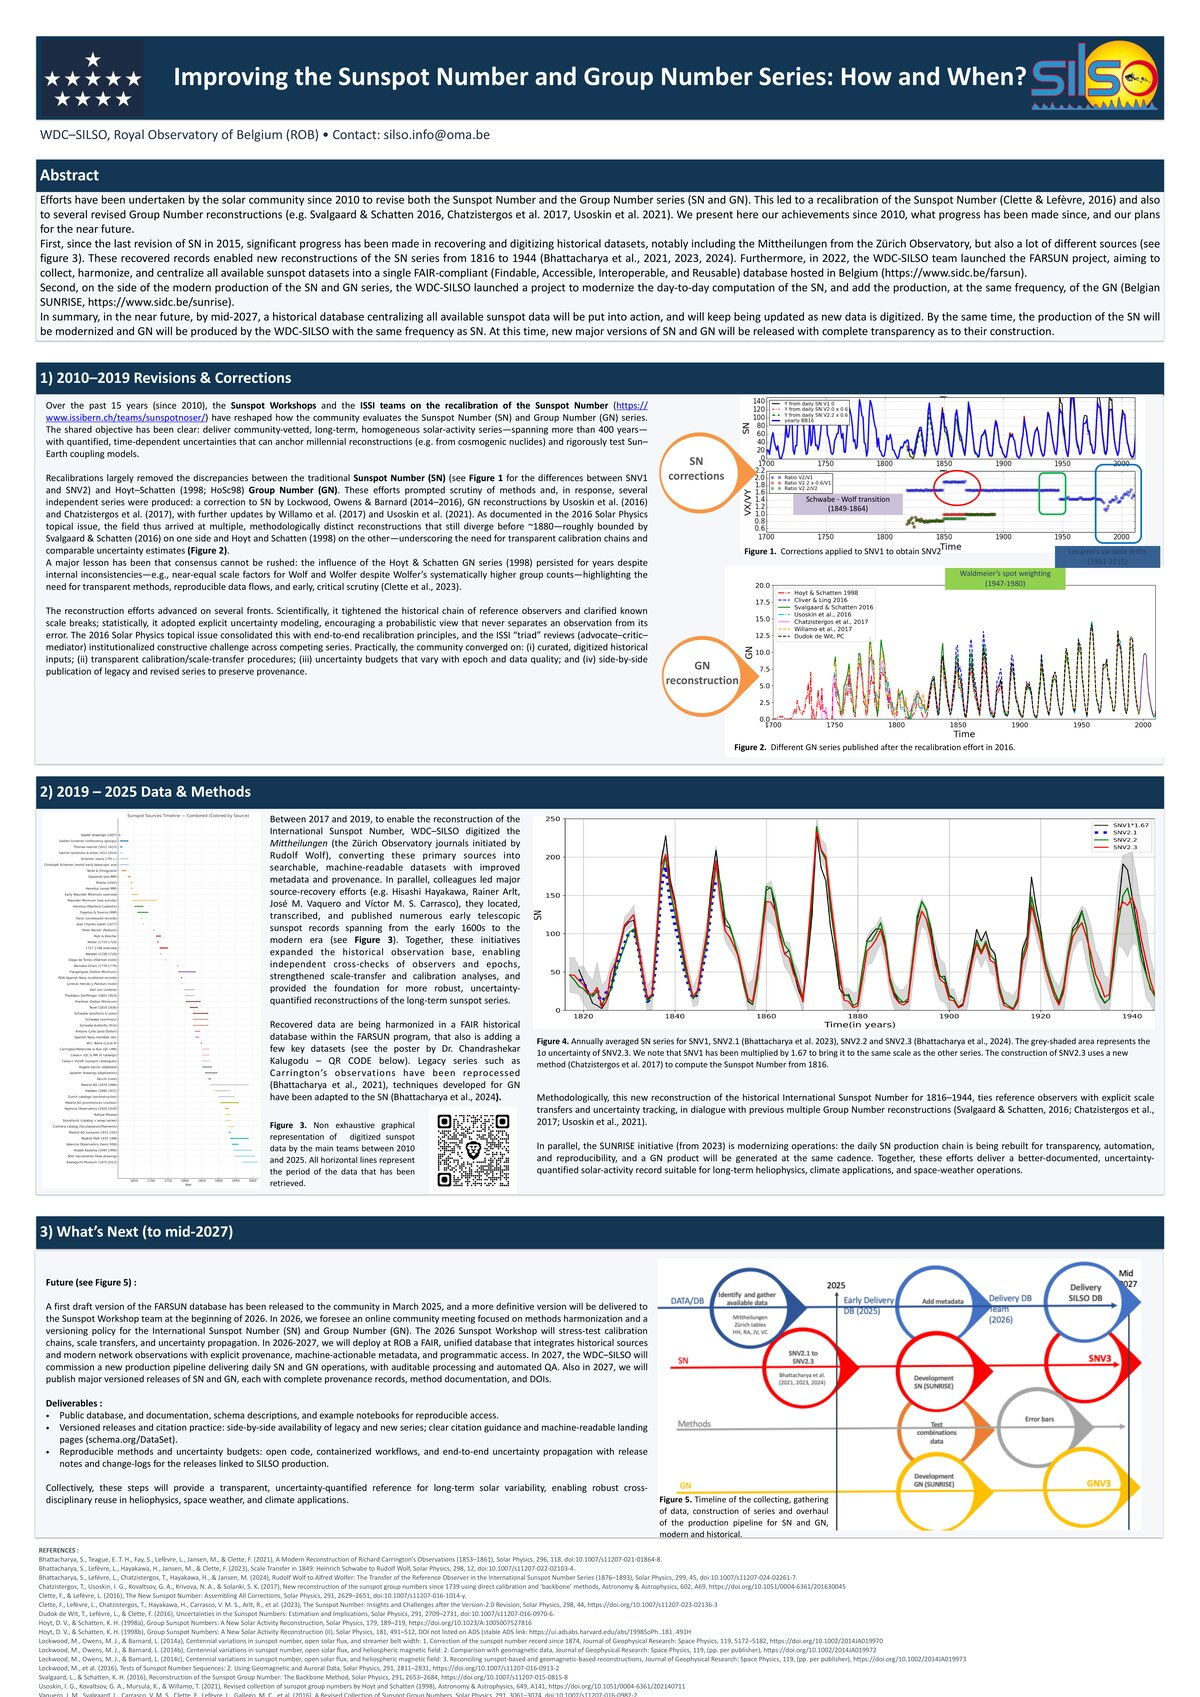
\includegraphics[width=\linewidth]{docs/SNGN_Poster_LLefevre_ESWW25_v1_web.jpg}
  \caption{\scriptsize Excerpt from the SN Next-Gen ESWW25 poster summarising governance pillars.}
\end{figure}
\end{columns}
\end{frame}

\section[Workflow]{Methodology}

\begin{frame}[t]{Four-Axis Workflow}
\begin{enumerate}
  \item \callout{Gather}{Locate and digitise dispersed historical sources (Wolf's \emph{Mittheilungen}, Zürich tables, Gruithuisen ledgers, Adams drawings).}
  \item \callout{Process}{Blend handwriting/OCR engines (Transkribus) with manual keying for fragile tables and drawings.}
  \item \callout{Validate}{Reconcile observer IDs, calendars, and counting conventions; propagate spotless-day confidence levels.}
  \item \callout{Disseminate}{Release FAIR-ready datasets, APIs, and VO-compliant services with versioned uncertainties.}
\end{enumerate}

\begin{center}
  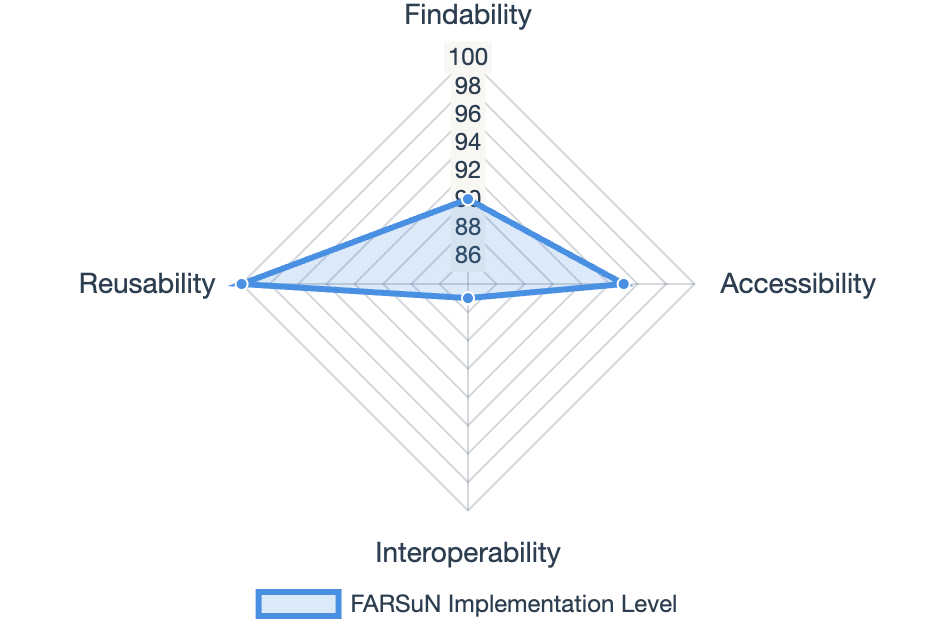
\includegraphics[width=0.5\linewidth]{./figures/fair_radar.png}
\end{center}
\end{frame}

\begin{frame}[t]{Quality Gates and Tooling}
\begin{columns}[T,onlytextwidth]
\column{0.5\linewidth}
\textbf{Verification}
\begin{itemize}
  \item Dual review of Adams and Gruithuisen counts before ingest.
  \item Cross-matching against Wolf and SILSO indices to flag drifts.
  \item Automated scripts check metadata completeness and naming standards.
\end{itemize}

\column{0.5\linewidth}
\textbf{Toolchain}
\begin{itemize}
  \item Transkribus handwriting models + manual correction interface.
  \item Python pipelines (Git-tracked) orchestrating OCR, QC, and format exports.
  \item Planned citizen science portal with training sets for Kurrent transcription.
\end{itemize}
\end{columns}
\end{frame}

\begin{frame}[t]{Data Pipeline to SN~V3}
\begin{enumerate}
  \item Curate daily group/spot counts with provenance-rich metadata.
  \item Solve observer response curves to harmonise scales over centuries.
  \item Aggregate to monthly, yearly, and hemispheric indices with propagated uncertainties.
  \item Benchmark against SN~V2, satellite-era proxies, and reconstructions to validate corrections.
\end{enumerate}

\begin{center}
  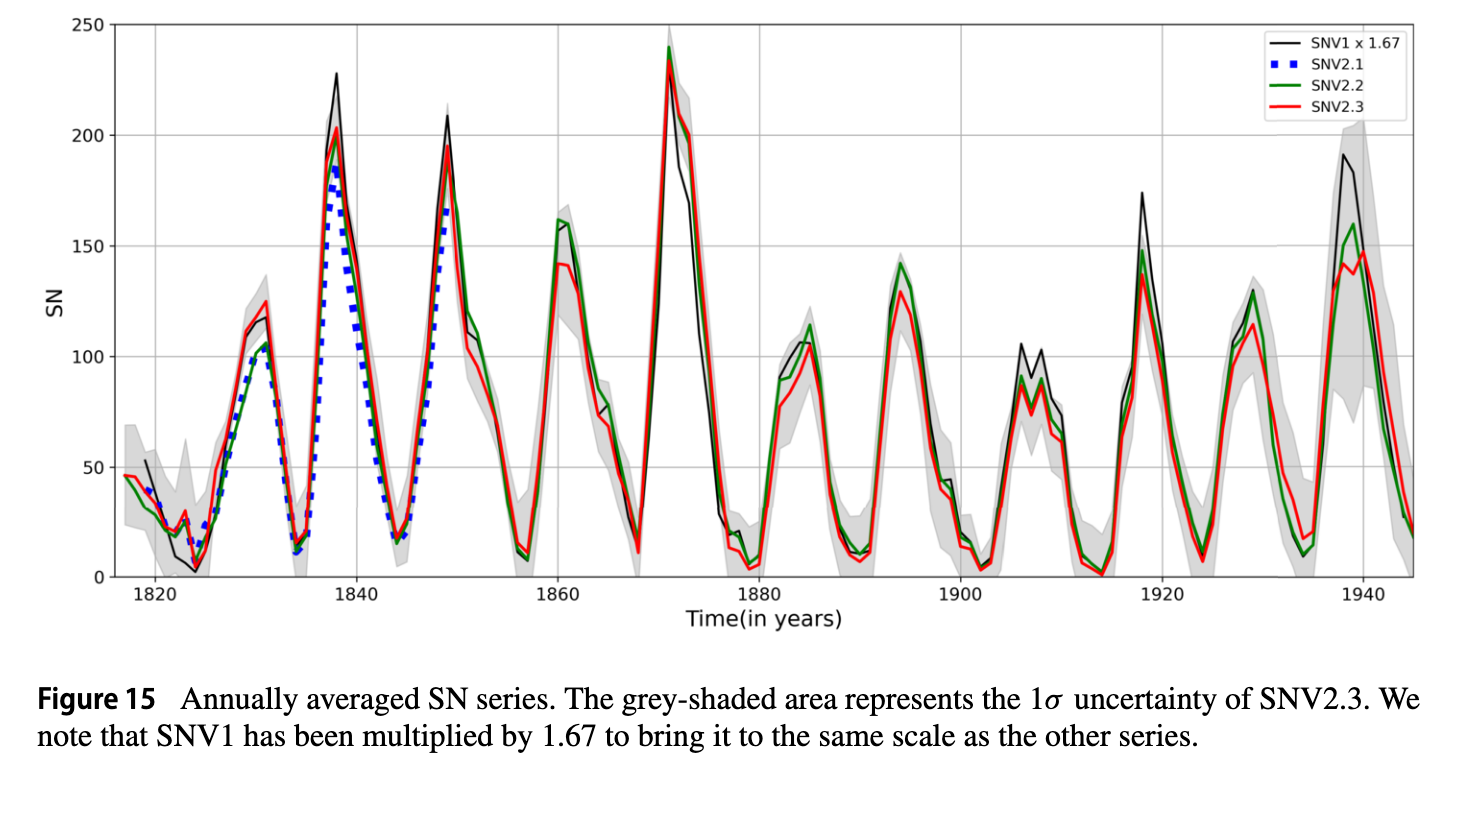
\includegraphics[width=0.7\linewidth]{./figures/comparison_panel.png}
\end{center}
\end{frame}

\section[Data]{Historical Assets}

\begin{frame}[t]{Zürich Tables — Summary}
\small
\begin{itemize}
  \item Daily ledgers from the Eidgenössische Sternwarte Zürich (1945–1979) capturing raw G/S counts, k-factors, and observing notes.
  \item Core digitisation complete; rich metadata encoded through 1959 with templates handling layout shifts across decades.
  \item QC reconciles observer aliases, cross-checks rubrics versus scans, and flags anomalies around the 1947 discontinuity.
  \item Next steps: finish 1951–1979 metadata, ingest 1980 bridging material, publish observer authority file, and expose VO/EPN-TAP products.
\end{itemize}

\vspace{0.6em}
\scriptsize Source: zurich\_tables.qmd.
\end{frame}

\begin{frame}[t]{Zürich Tables — Ledger Excerpt}
\centering
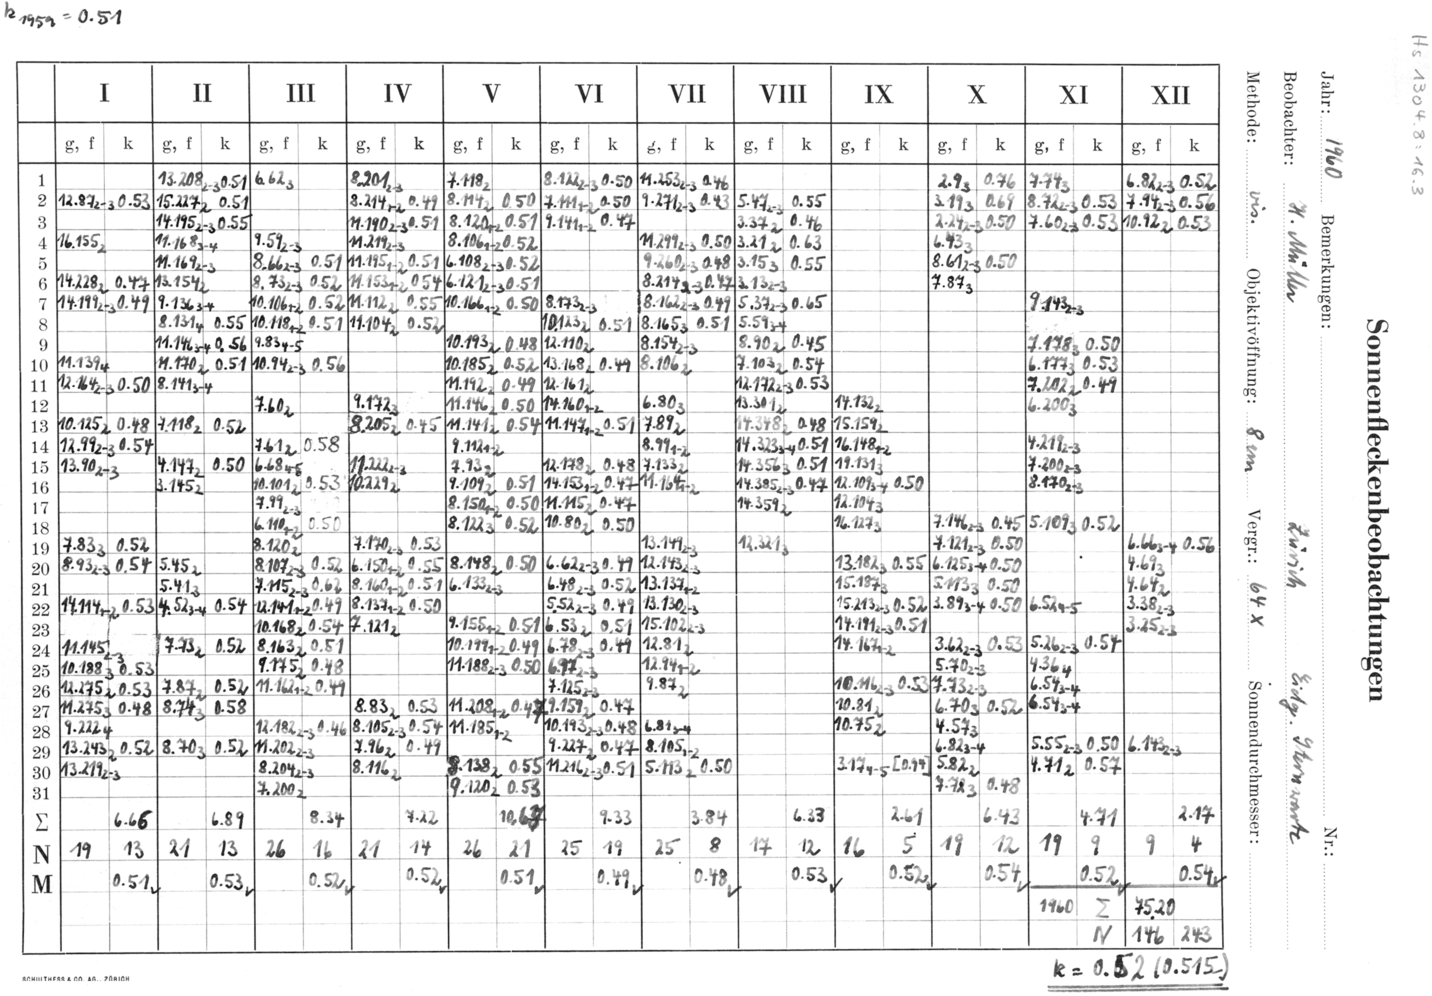
\includegraphics[width=0.8\linewidth]{zurich_tables.png}

\vspace{0.4em}
\scriptsize Sample Waldmeier-era ledger page showing per-observer counts and k-factor selections.
\end{frame}

\begin{frame}[t]{Mittheilungen — Summary}
\small
\begin{itemize}
  \item Rudolf Wolf’s printed annual reports (1610–1918) aggregate daily GN/NS tallies, observer IDs, and annotations across Europe.
  \item Fully digitised and mapped to observers/rubrics; provenance fields capture volume and page for reproducibility.
  \item QC pipelines flag GN/S anomalies, reconcile aliases, and cross-compare against Adams extractions to catch residual errors.
  \item Upcoming focus: calibrate Wolf–Wolfer overlaps, enrich observing-condition metadata, and publish VO/EPN-TAP services.
\end{itemize}

\vspace{0.6em}
\scriptsize Source: mittheilungen\_data-1800.qmd.
\end{frame}

\begin{frame}[t]{Mittheilungen — Printed Tables}
\centering
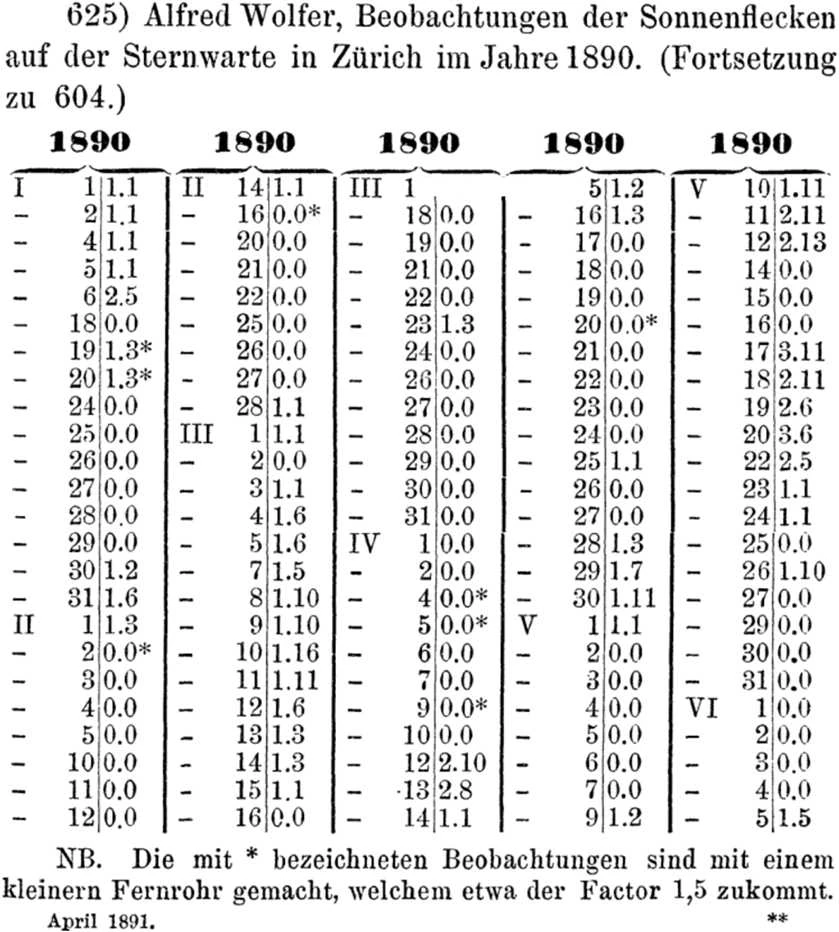
\includegraphics[width=0.75\linewidth]{mittheilungen_sample.png}

\vspace{0.4em}
\scriptsize Mid-19th-century \emph{Mittheilungen} page showing multi-observer entries and Wolf number columns.
\end{frame}

\begin{frame}[t]{C. H. Adams Drawings — Summary}
\small
\begin{itemize}
  \item Dense run of full-disk drawings (1819–1823) with NG/NS counts, spotless flags, and direct vs reflection viewing modes.
  \item 338 folios produce 1,056 dated entries, adding ~650 spotless statements beyond Zürich compilations.
  \item Processing pipeline dewarps sketches, harmonises notation, and links provenance for integration into the FARSuN database.
  \item Near-term work: finalise coverage calendar, publish comparison logs, and release v1 dataset with uncertainty annotations.
\end{itemize}

\vspace{0.6em}
\scriptsize Source: adams.qmd.
\end{frame}

\begin{frame}[t]{C. H. Adams Drawings — Example Folio}
\centering
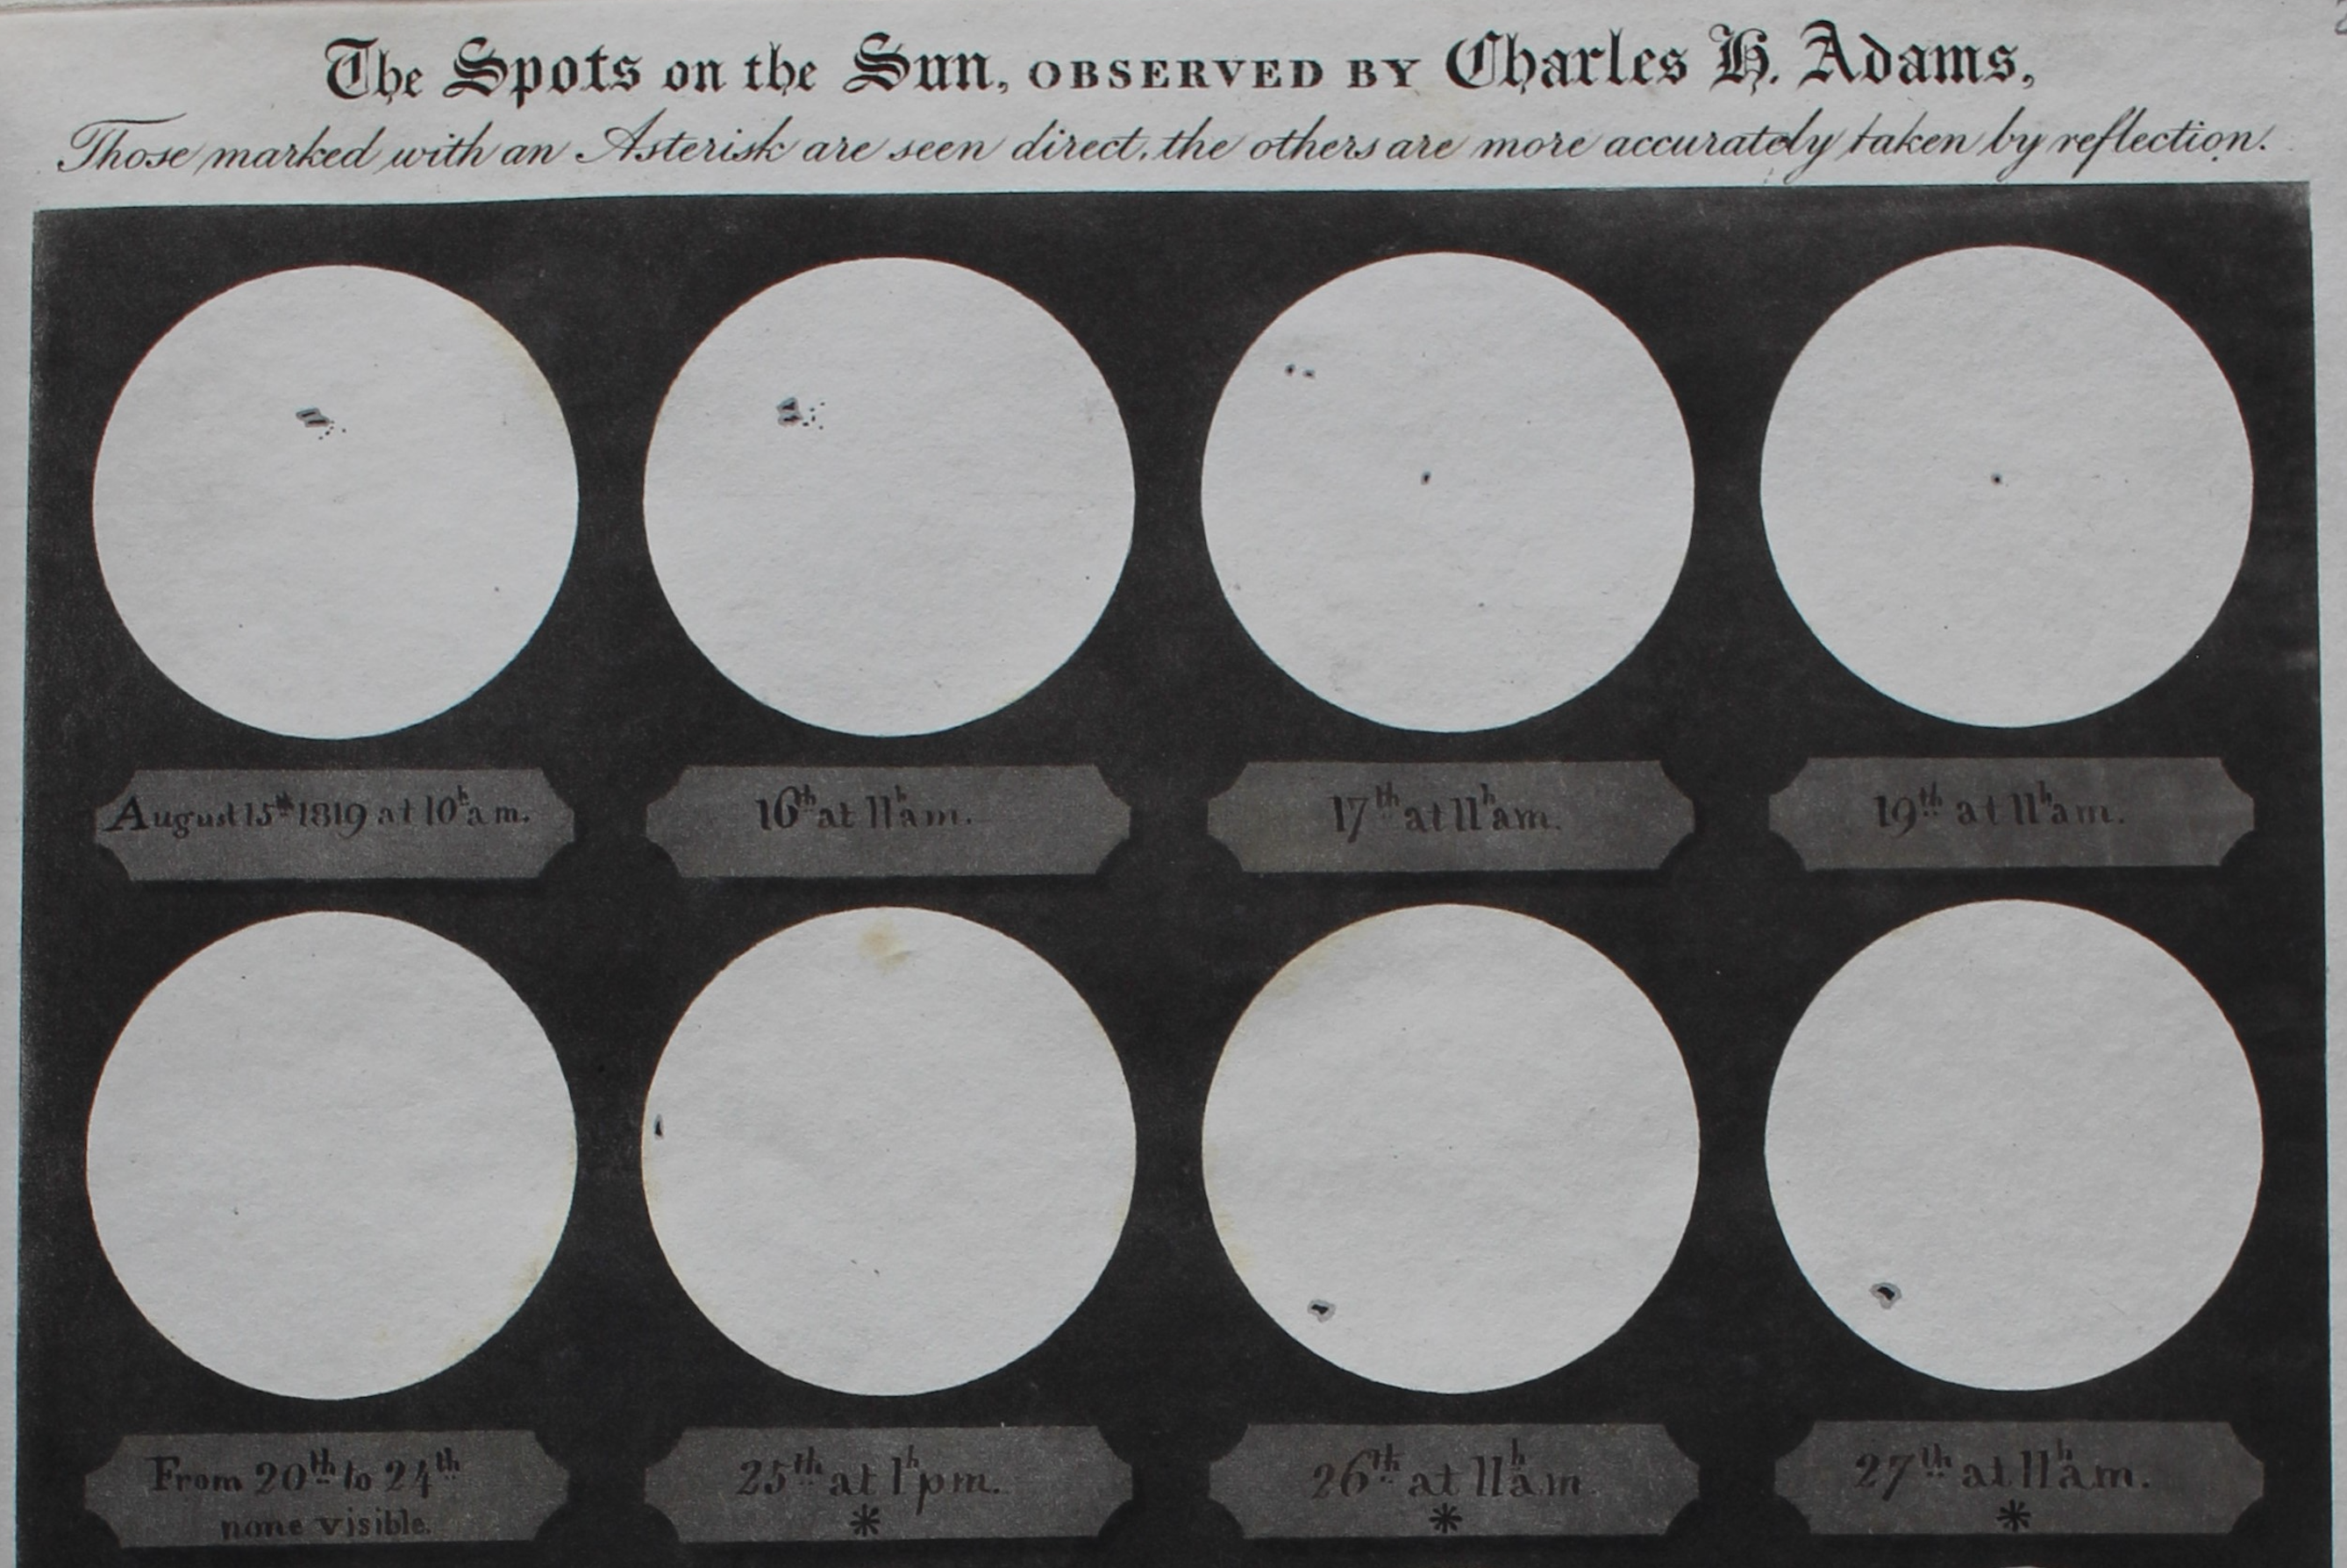
\includegraphics[width=0.8\linewidth]{adams_example.png}

\vspace{0.4em}
\scriptsize Annotated drawing highlighting group layout, spotless notes, and viewing method for SN V3 calibration.
\end{frame}

\begin{frame}[t]{Gruithuisen Manuscripts — Summary}
\small
\begin{itemize}
  \item Munich-based notebooks (1817–1849) combining textual weather notes and sketches written in Kurrent script.
  \item All scans prepared; Transkribus workflow plus dual QC validates transcription accuracy and counts.
  \item Supplies Dalton-Minimum coverage, spotless/active flags, and environmental context for bias analysis.
  \item Pending tasks: finish survey pass, produce provisional NG/NS with uncertainties, and publish VO-ready tables.
\end{itemize}

\vspace{0.6em}
\scriptsize Source: gruithuisen.qmd.
\end{frame}

\begin{frame}[t]{Gruithuisen Manuscripts — Sample Page}
\centering
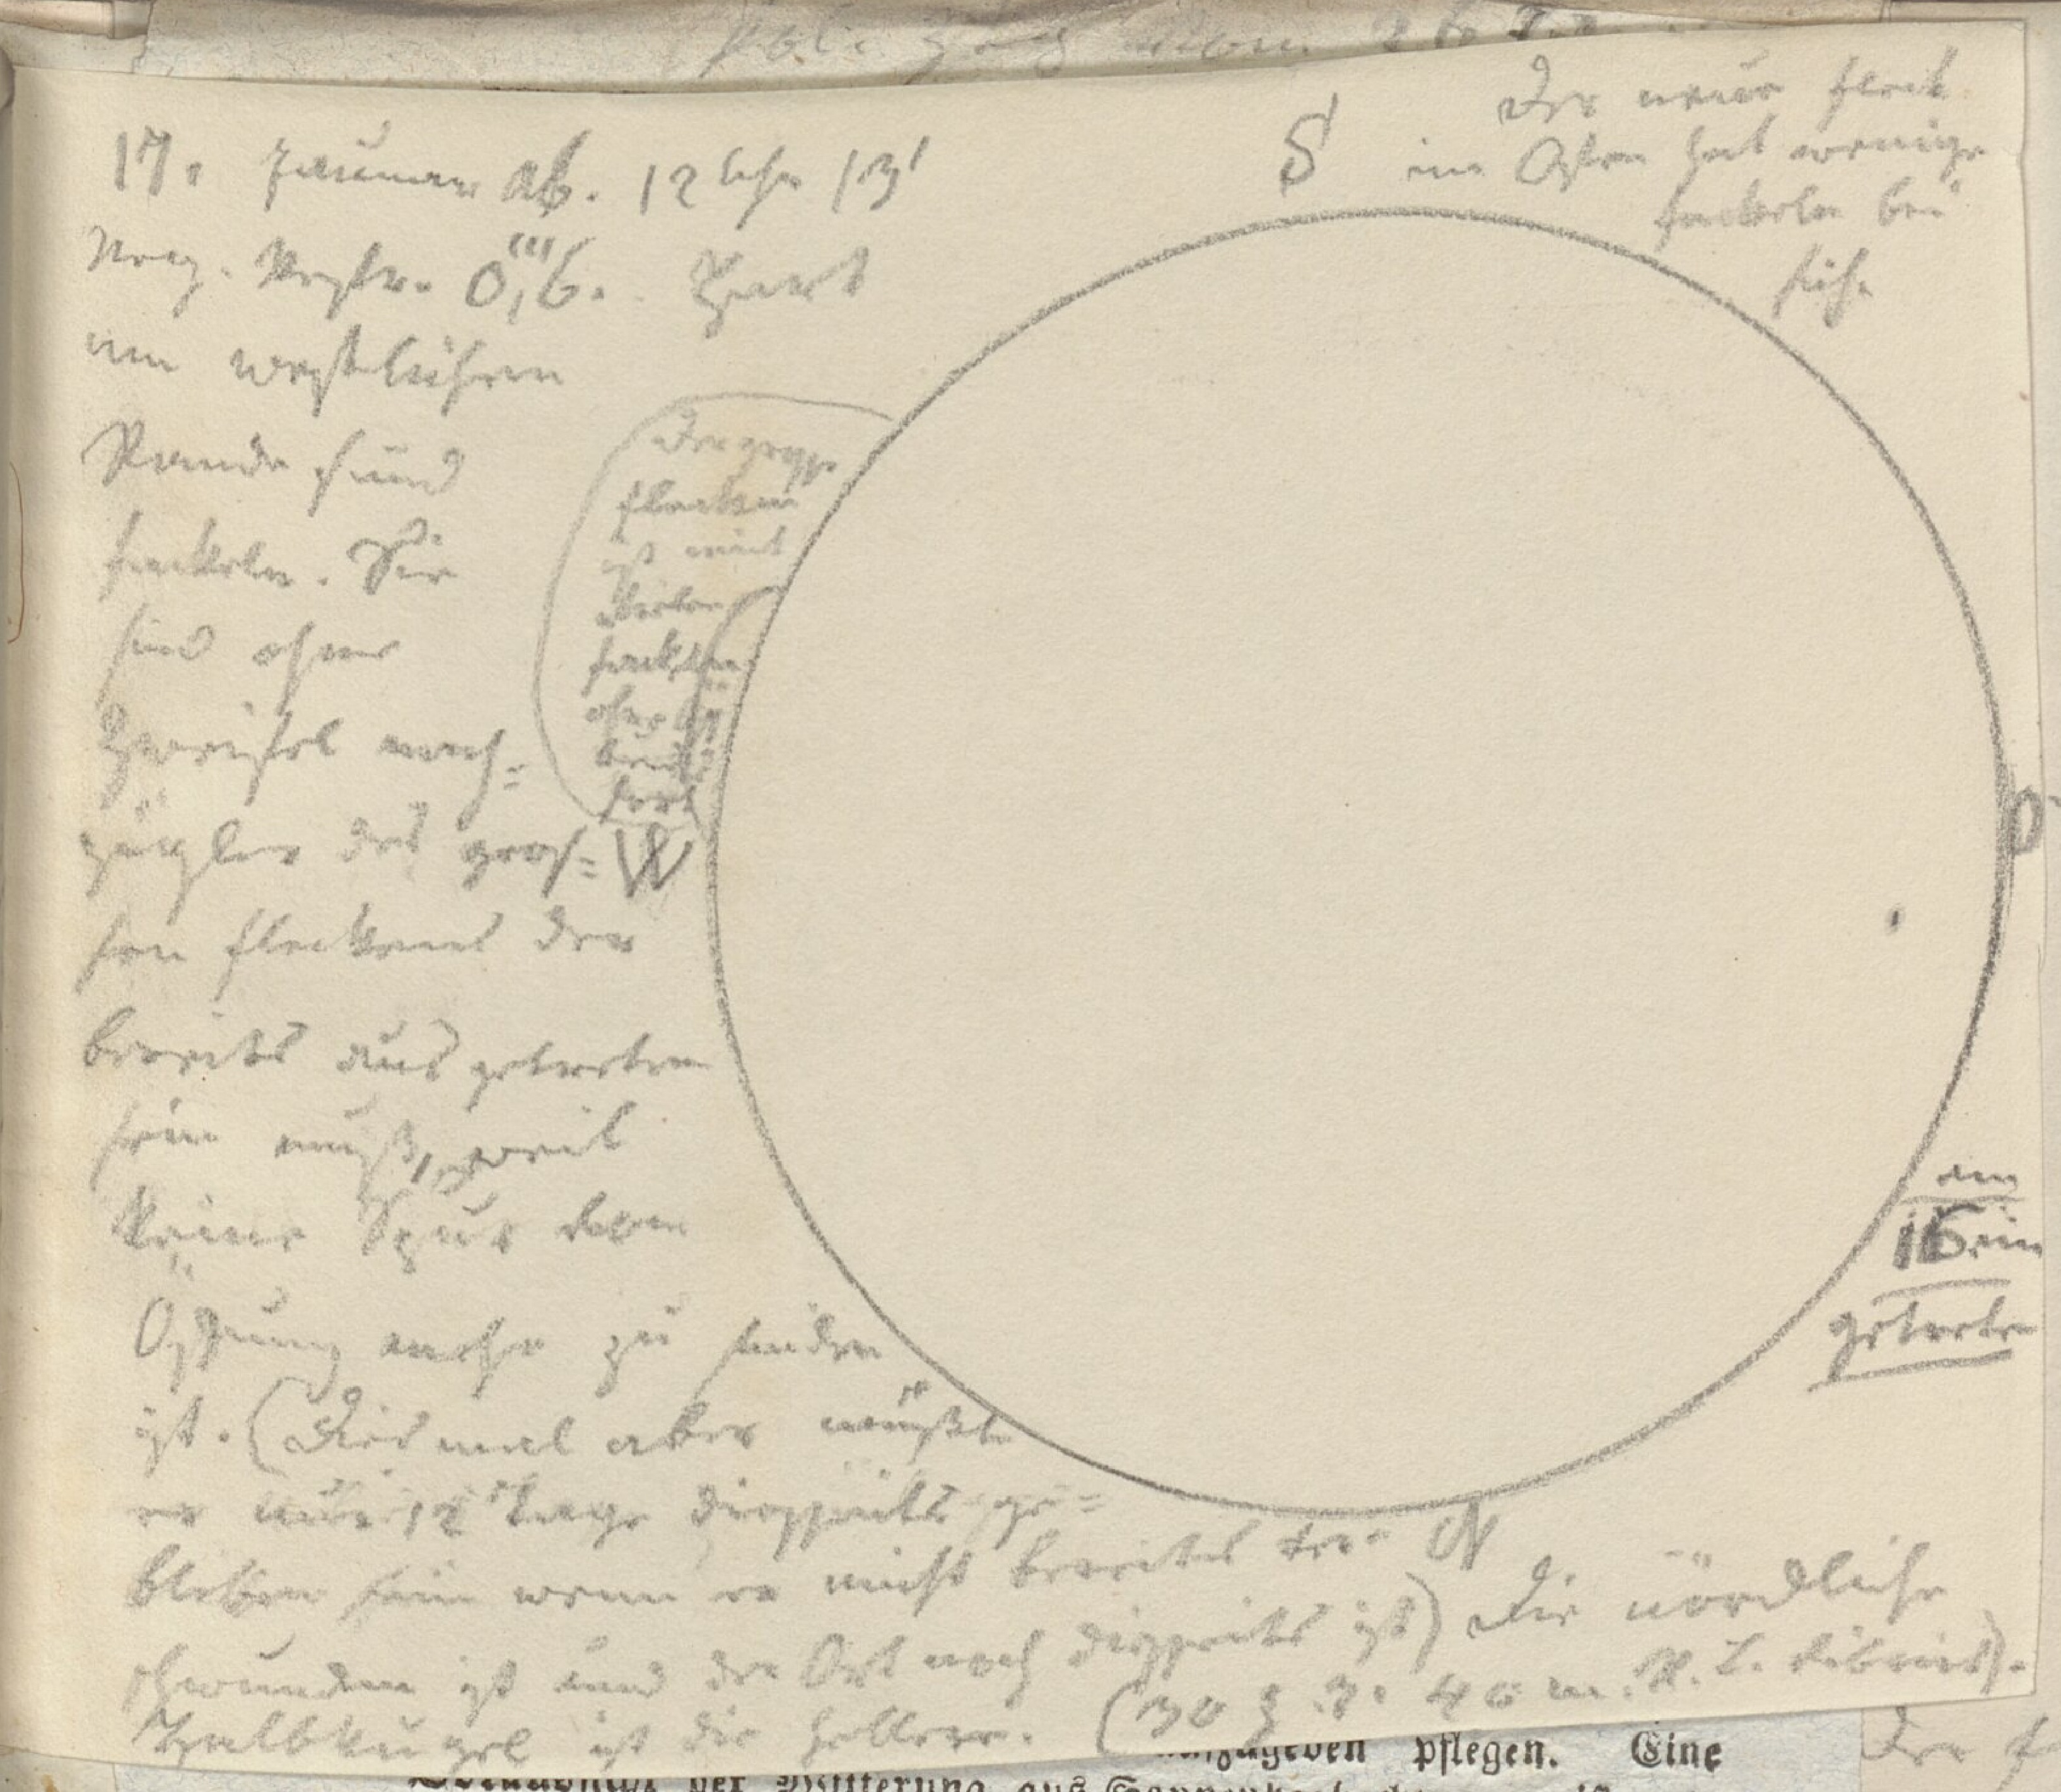
\includegraphics[width=0.8\linewidth]{Gruithuisen_Sample2.jpg}

\vspace{0.4em}
\scriptsize Manuscript excerpt coupling weather commentary with sunspot sketches; dual QC mitigates transcription ambiguity.
\end{frame}

\begin{frame}[t]{Augustin Stark Ledgers — Summary}
\small
\begin{itemize}
  \item Printed narratives (~1813–1835) capturing morphology, limb distances, and counts during the Dalton/post-Dalton era.
  \item OCR plus prompt-guided extraction converts Fraktur prose into structured NG/NS data with provenance metadata.
  \item Offers spotless-day coverage and qualitative QC cues to support SN V3.1/V4 calibration chains.
  \item Next steps: finalise bibliography/page mappings, publish extraction taxonomy, and integrate derived scaling priors.
\end{itemize}

\vspace{0.6em}
\scriptsize Source: stark.qmd.
\end{frame}

\begin{frame}[t]{Augustin Stark Ledgers — Page Extract}
\centering
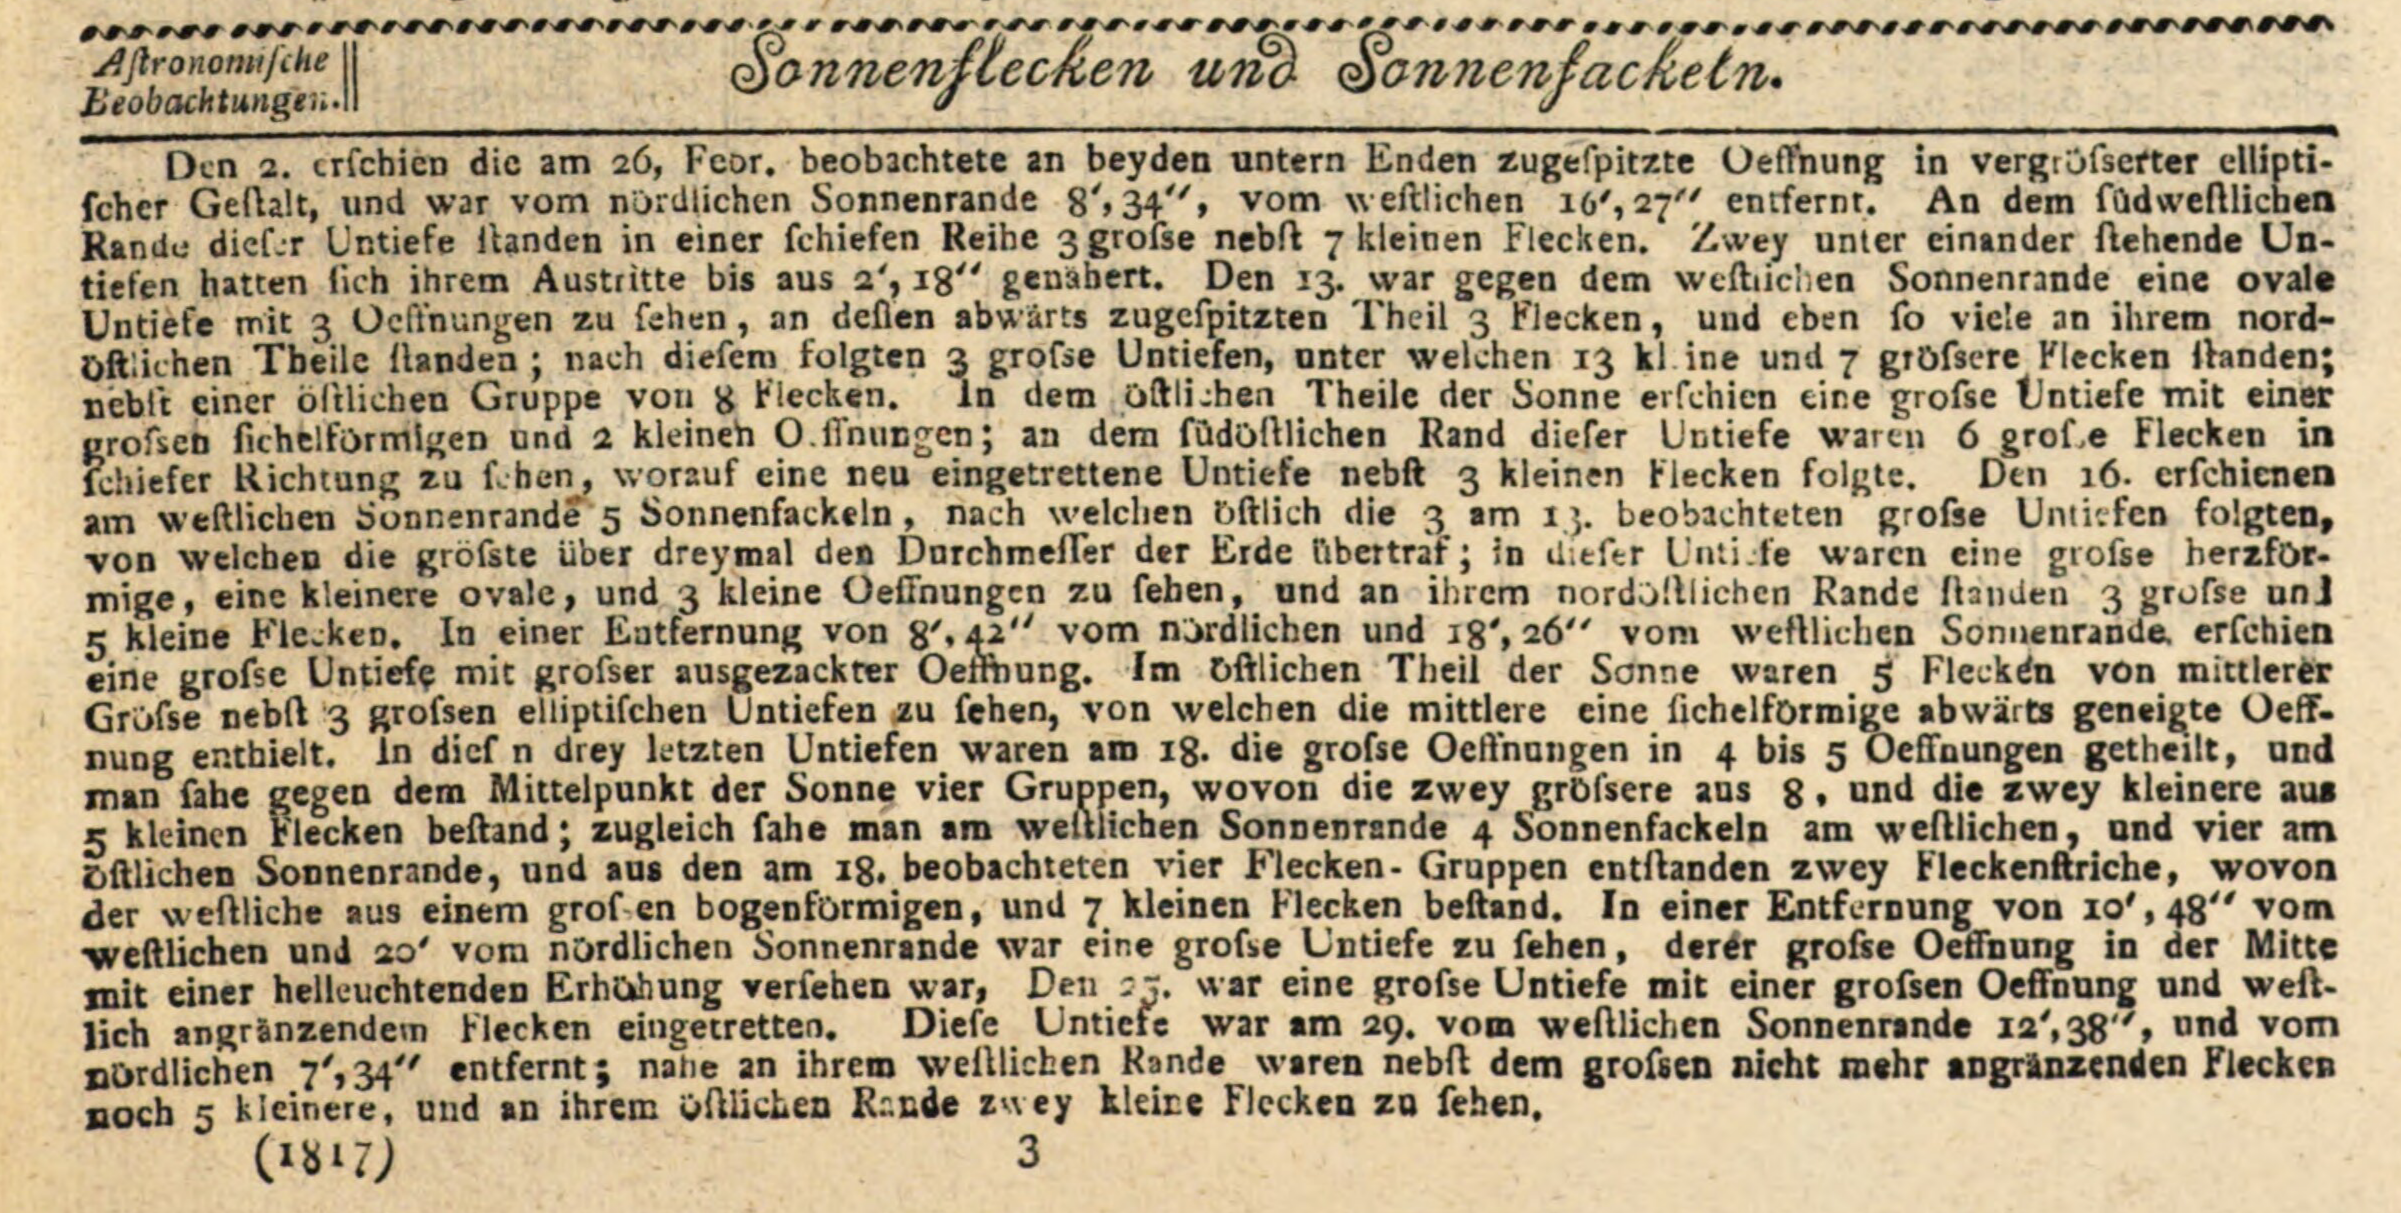
\includegraphics[width=0.78\linewidth]{Stark_Sample1.png}

\vspace{0.4em}
\scriptsize Example Stark entry with narrative descriptors and counts prepared for OCR-driven ingestion.
\end{frame}

\begin{frame}[t]{Observer Coverage}
\begin{figure}
  \centering
  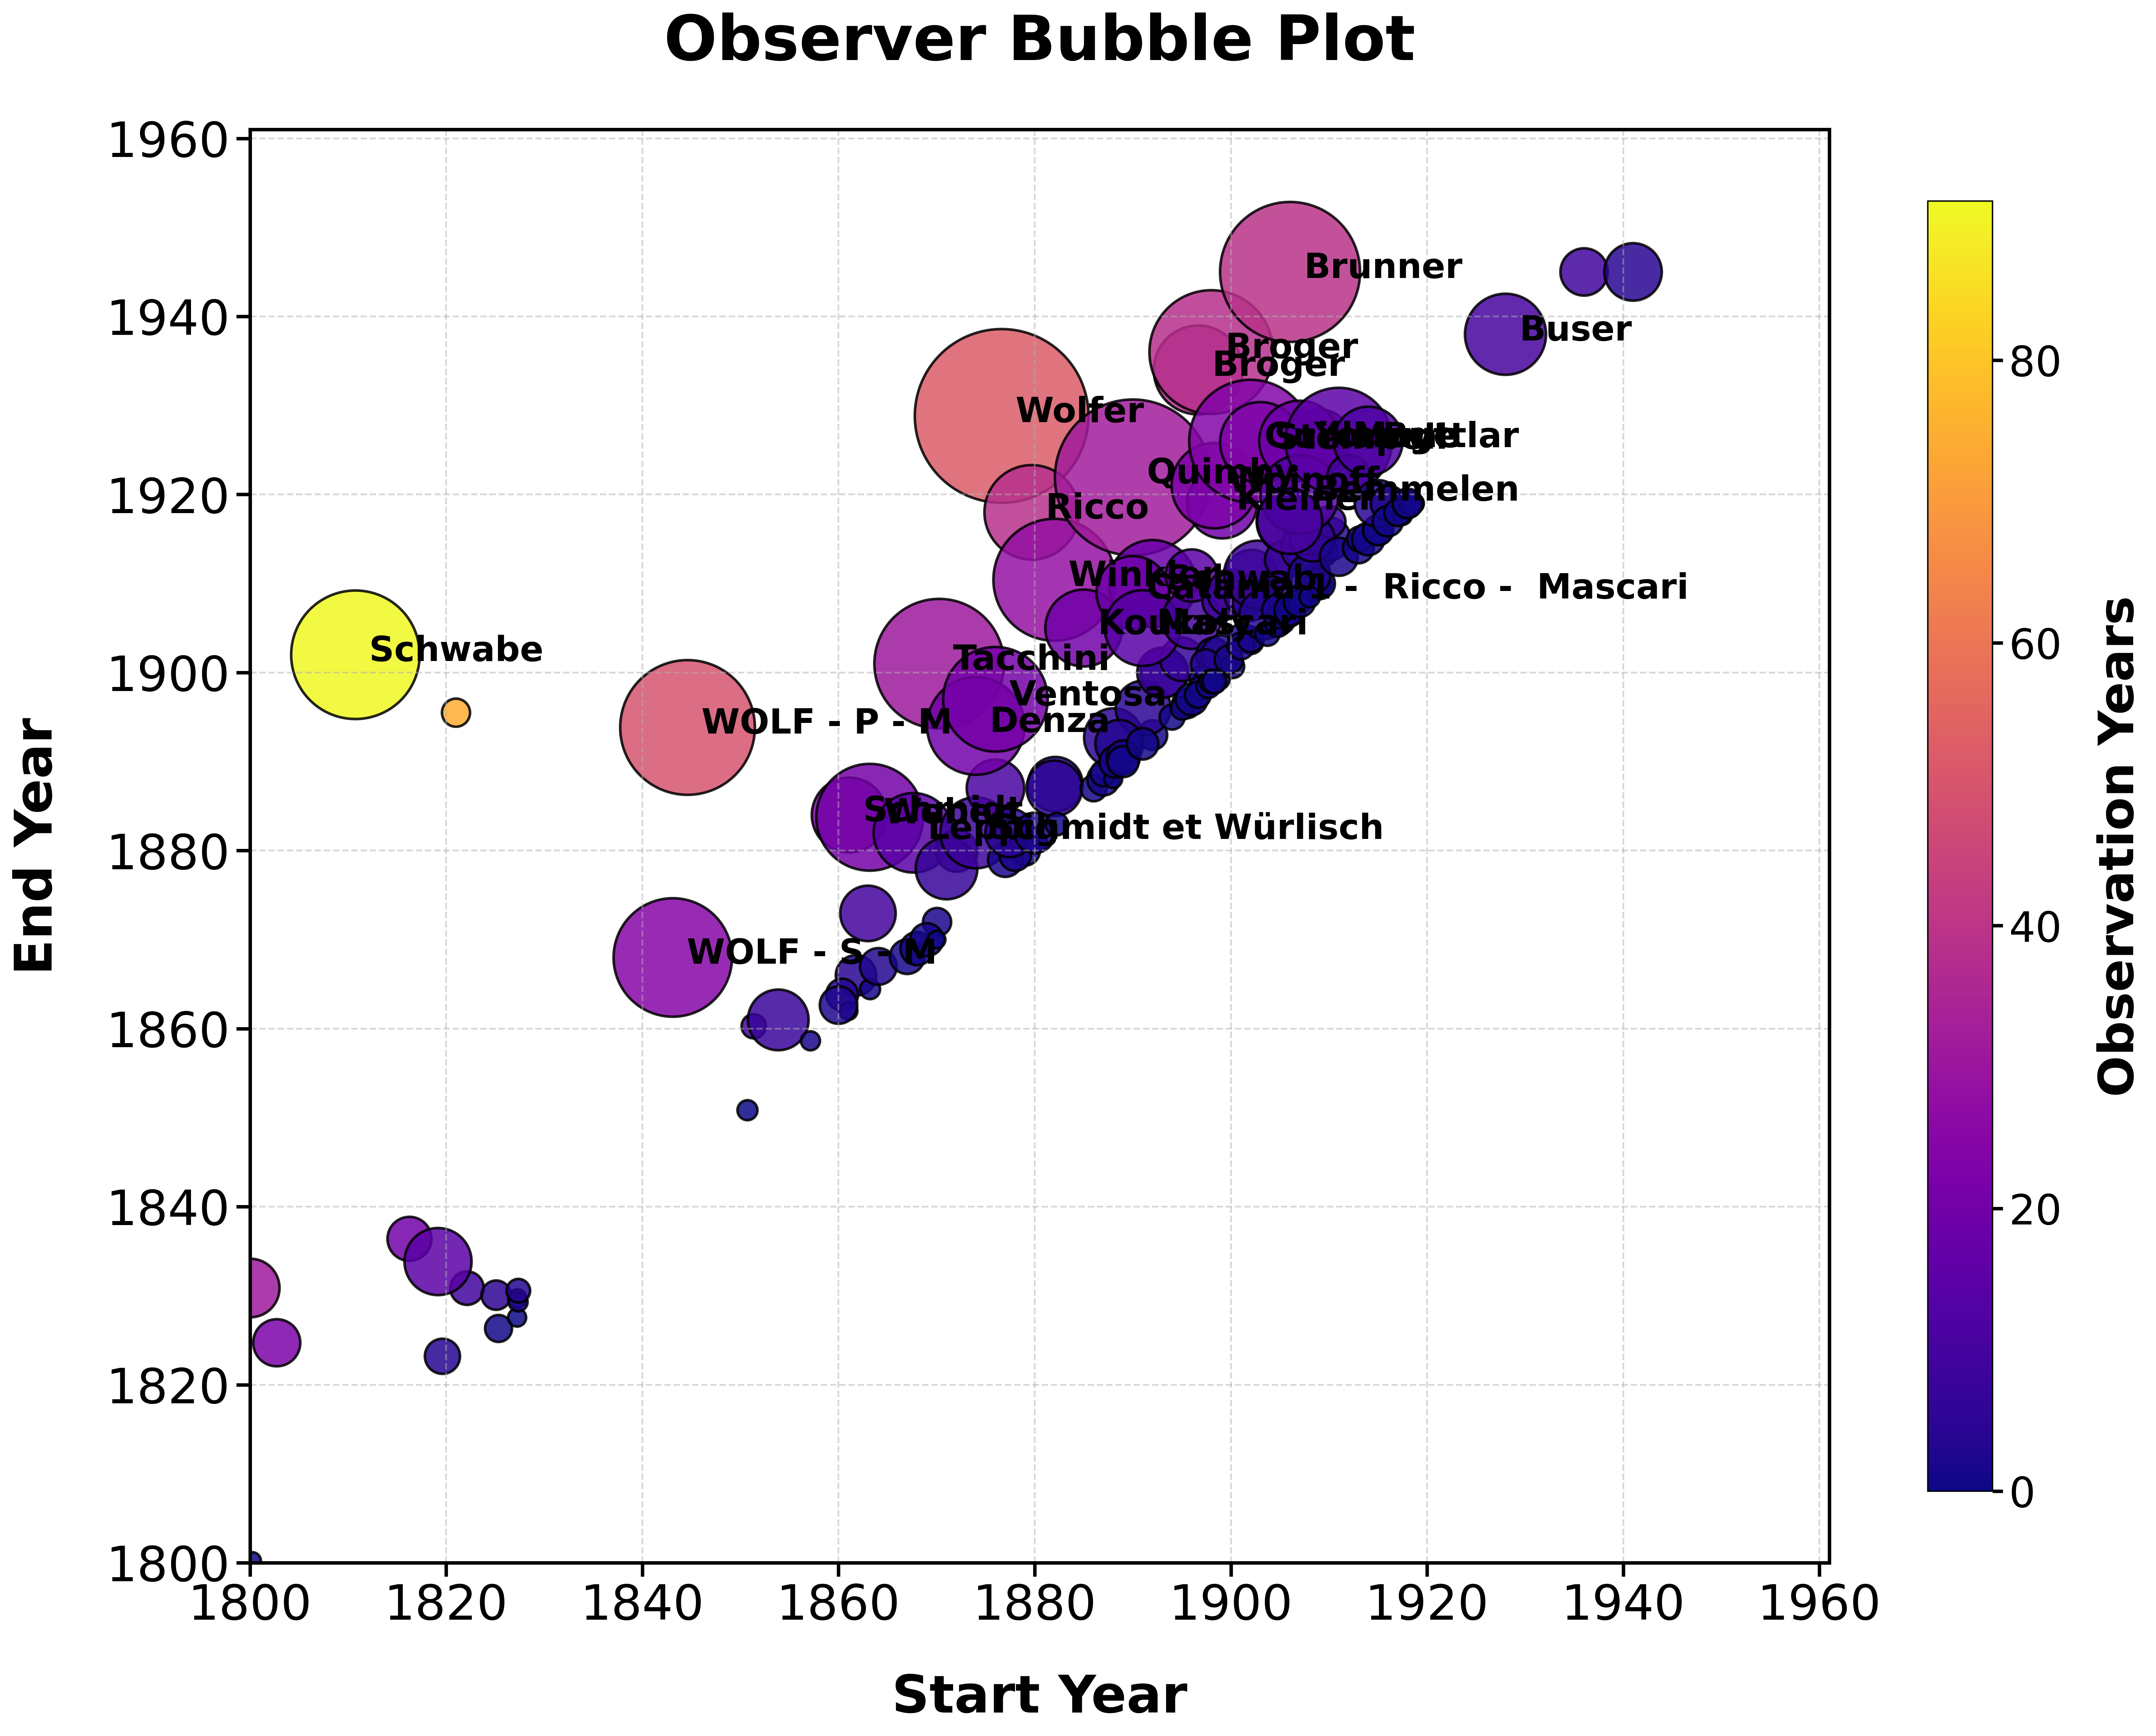
\includegraphics[width=0.65\linewidth]{observer_bubbles_poster_v2.png}
  \vspace{0.3em}
  {\scriptsize Bubble size = total observations; colour encodes observing years (Source: FARSuN observer coverage dashboard).}
\end{figure}
\end{frame}

\section[Impact]{Science Impact}

\begin{frame}[t]{Addressing Core Challenges}
\begin{columns}[T,onlytextwidth]
\column{0.5\linewidth}
\textbf{Data hurdles}
\begin{itemize}
  \item Deciphering 19th-century \emph{Kurrent} handwriting and marginalia.
  \item Normalising heterogeneous formats (drawings, tables, narrative notes).
  \item Tracking provenance from scanned folio to released dataset.
\end{itemize}

\column{0.5\linewidth}
\textbf{Mitigations}
\begin{itemize}
  \item Specialist training, handwriting models, and dual QC.
  \item Schema mapping + metadata vocabularies across archives.
  \item Git-backed pipelines with audit trails and uncertainty flags.
\end{itemize}
\end{columns}
\end{frame}

\begin{frame}[t]{Benefits for the Community}
\begin{columns}[T,onlytextwidth]
\column{0.48\linewidth}
\callout{Forecasting}{Bias-reduced SN~V3 improves solar cycle prediction skill and operational space weather baselines.}
\vspace{1em}
\callout{Climate}{Validated long-term forcing records refine Earth system and climate models.}

\column{0.48\linewidth}
\callout{Citizen science}{Public transcription portal accelerates data recovery and outreach.}
\vspace{1em}
\callout{Open science}{FAIR datasets, APIs, and reproducible notebooks catalyse external research.}
\end{columns}
\end{frame}

\section[Outlook]{Path Ahead}

\begin{frame}[t]{2025 Roadmap}
\begin{itemize}
  \item Launch citizen-science transcription pilot with curated training sets.
  \item Finalise Zürich metadata encoding and close remaining digitisation gaps.
  \item Publish SN~V3 release notes with full uncertainty budget and API endpoints.
  \item Expand collaborations (ROB, Nagoya, UCLouvain) for cross-validation and joint publications.
\end{itemize}
\begin{center}
  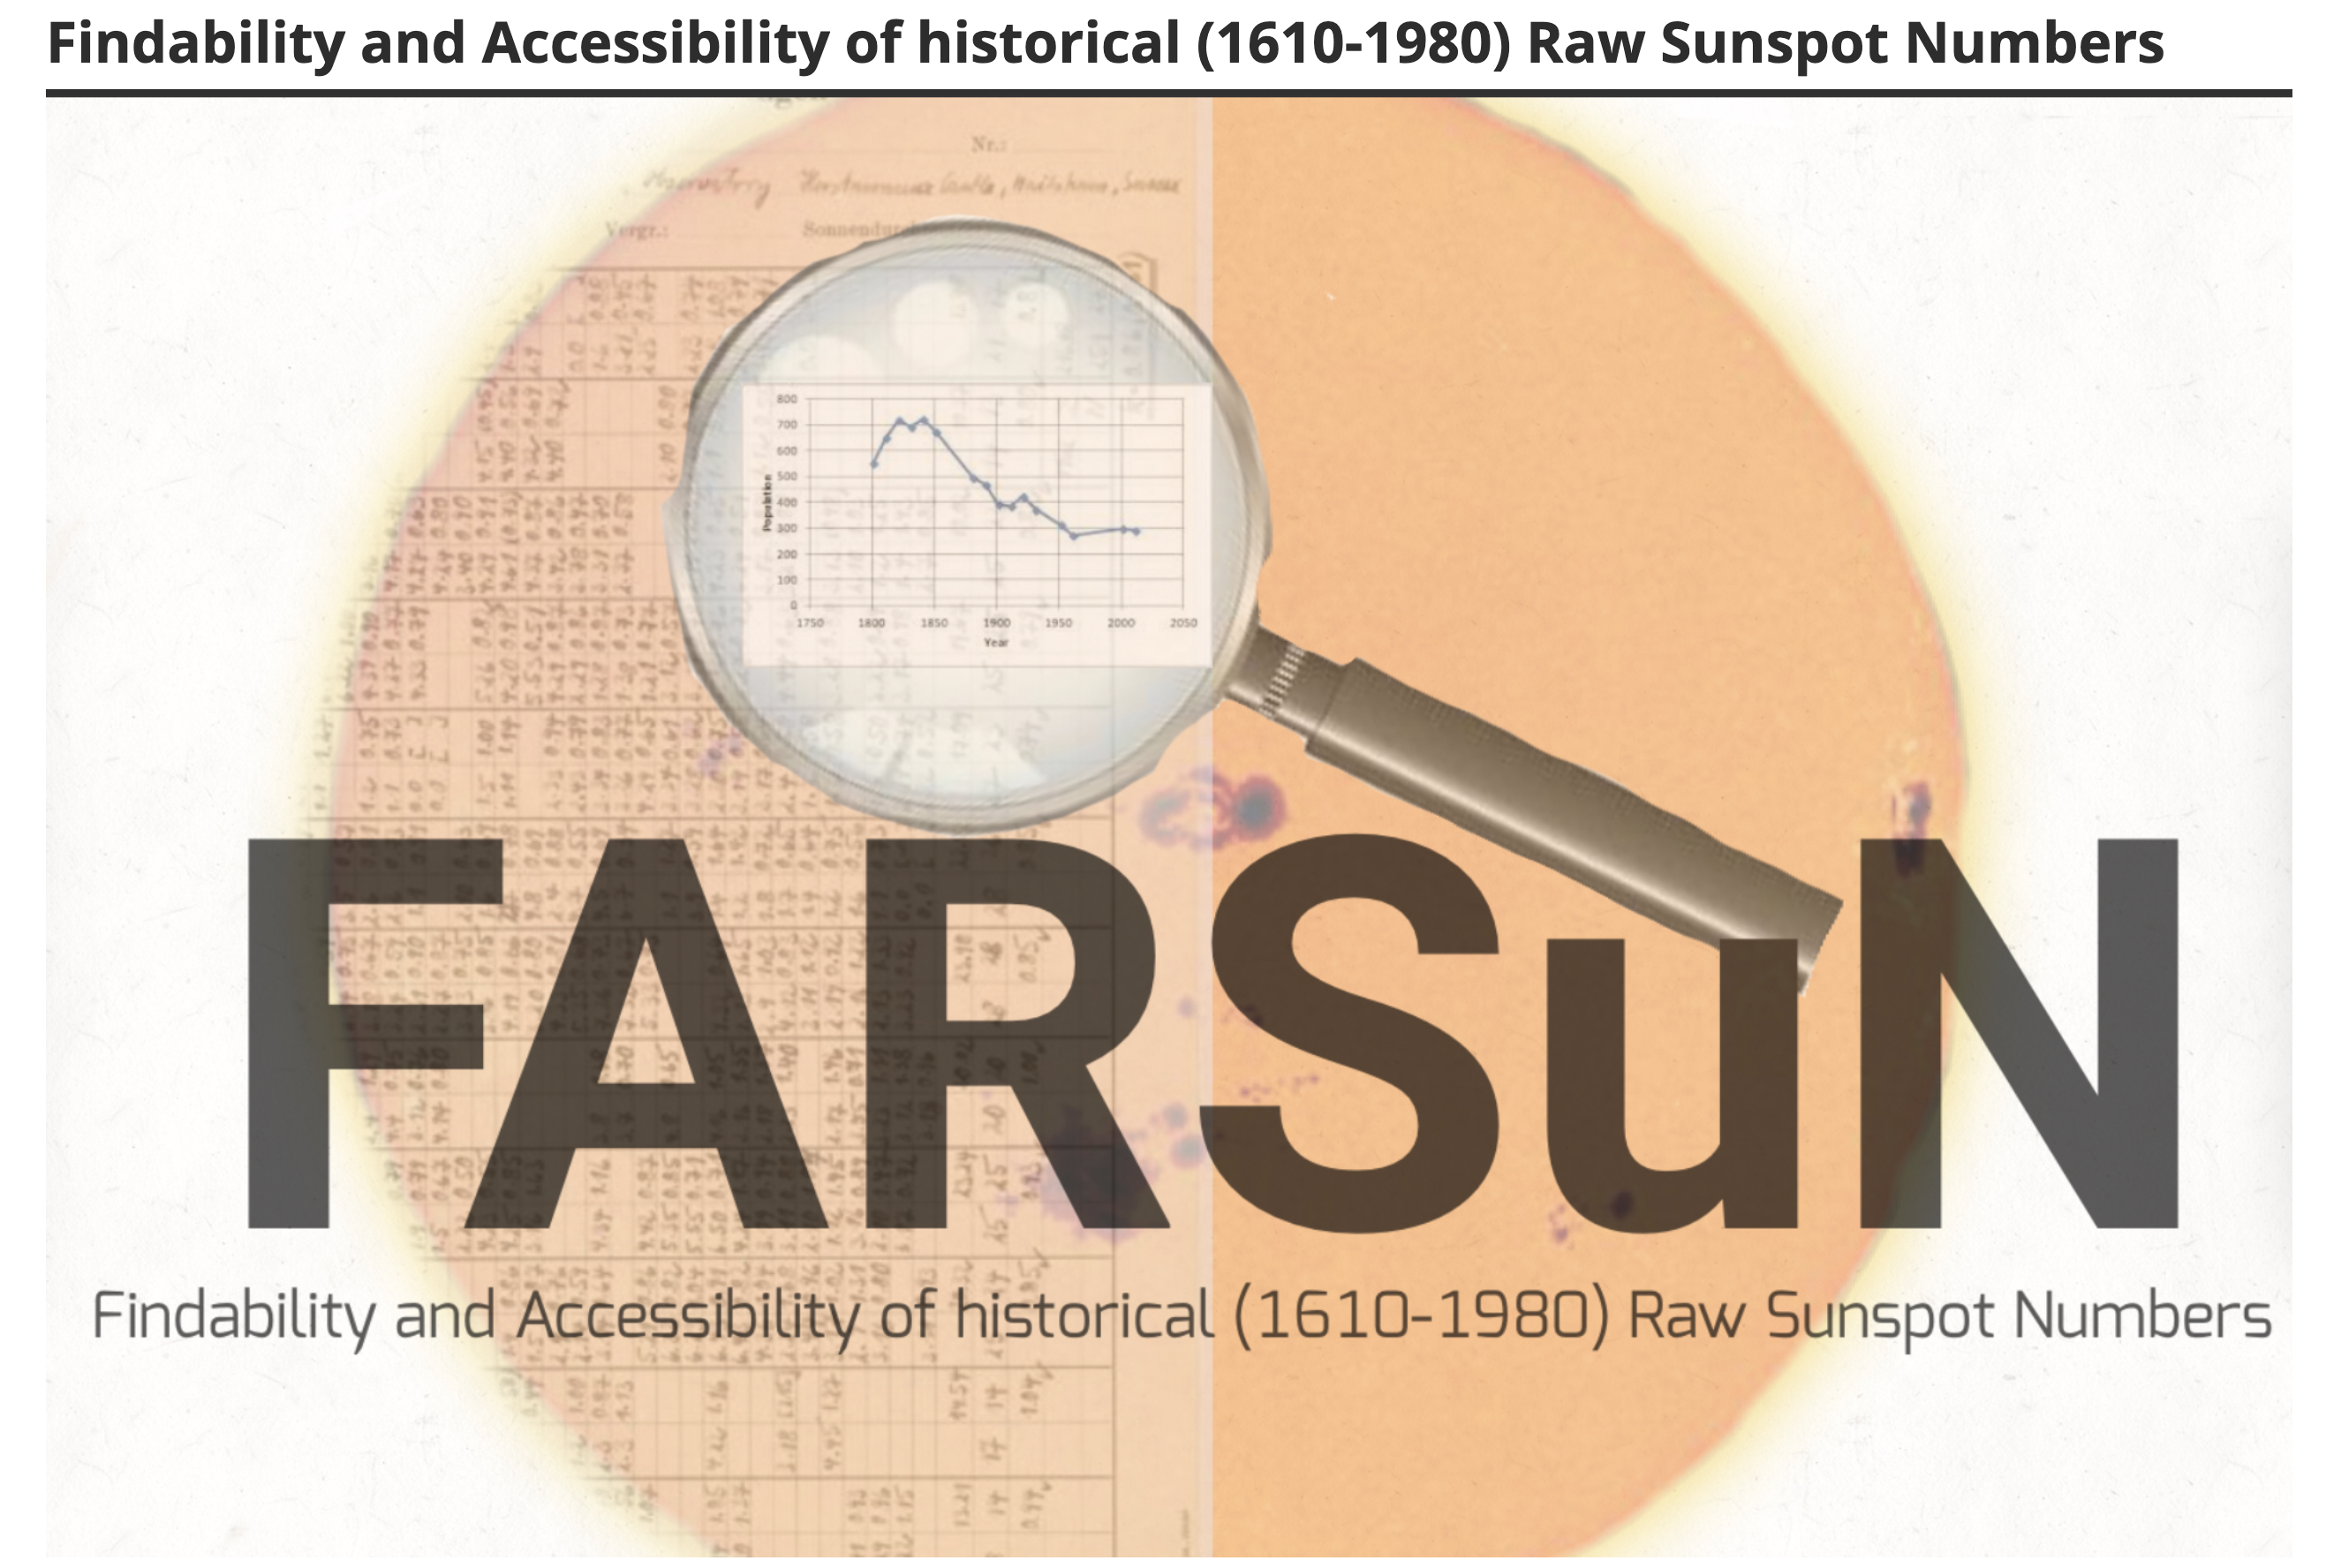
\includegraphics[width=0.45\linewidth]{./figures/ack_.png}
\end{center}
\end{frame}

\section*{Q\&A}

\begin{frame}
\centering
\Huge\color{royal}{Questions?}

\vspace{1em}
\small \href{mailto:silso.info@observatory.be}{silso.info@observatory.be} \quad | \quad \url{https://www.sidc.be/silso/}
\end{frame}

\end{document}
